\documentclass[11pt,a4paper]{jsarticle}

\makeatletter

%%% 個人設定 
\usepackage{amsmath,amssymb}
\usepackage{amsthm}
\usepackage{graphicx}

\usepackage[scaled]{helvet}

\bibliographystyle{plain}

\newcommand{\R}{\mathbf R}
\newcommand{\N}{\mathbf N}
\newcommand{\Q}{\mathbf Q}
\newcommand{\Z}{\mathbf Z}
\newcommand{\D}{D}
\newcommand{\classP}{\mathsf{P}}
\newcommand{\classPSPACE}{\mathsf{PSPACE}}
\newcommand{\classNP}{\mathsf{NP}}
\newcommand{\classNumberP}{\mathsf{\#P}}
\newcommand{\classPH}{\mathsf{PH}}
\newcommand{\classPP}{\mathsf{PP}}
\newcommand{\classCH}{\mathsf{CH}}
\newcommand{\classSigma}{\mathsf{\Sigma}}
\newcommand{\quantC}{\mathsf{C}}

\newcommand{\OpIVP}{\mathit{ODE}}
\newcommand{\deltabox}{\delta _\square}
\newcommand{\deltaboxLip}{\delta _{\square \mathrm L}}
\newcommand{\classtwofont}[1]{\text{\bfseries \sffamily \upshape #1}}
\newcommand{\classFPSPACEtwo}{\classtwofont{FPSPACE}}
\newcommand{\classCHtwo}{\classtwofont{CH}}
\newcommand{\redW}{\leq _{\mathrm W}}
\newcommand{\classLip}{\mathrm C _{\mathrm L}}
\newcommand{\classC}{\mathrm C}

\theoremstyle{definition}
\newtheorem{theorem}{定理}[section]
\newtheorem{lemma}[theorem]{補題}
\newtheorem{definition}[theorem]{定義}

\renewcommand{\proofname}{\bf 証明} 

%%% 数式中の大文字ギリシャ文字を斜体化
\renewcommand{\Lambda}{\varLambda}
\renewcommand{\Gamma}{\varGamma}

%%% (i), (ii), (iii), (iv)
\def\theenumi{\roman{enumi}}
\def\labelenumi{(\theenumi)}

%%% 数式番号を(章.num) に
\renewcommand{\theequation}{\thesection.\arabic{equation}}
\@addtoreset{equation}{section}

%%% 表番号を 章.num に
\renewcommand{\thetable}{\thesection.\arabic{table}}
\@addtoreset{table}{section}

%%% 図番号を 章.num に
\renewcommand{\thefigure}{\thesection.\arabic{figure}}
\@addtoreset{figure}{section}

\makeatother

\title{滑らかな常微分方程式の計算量}

\author{%
\hspace*{7zw}% 良い子は真似してはいけません!
太田浩行\thanks{東京大学, \texttt{hota@is.s.u-tokyo.ac.jp}} 
\and
河村彰星\thanks{東京大学}%
\hspace*{7zw}% 良い子は真似してはいけません!
\and
マルチン・ツィーグラー\thanks{Martin Ziegler, ダルムシュタット工科大学}
\and
カルステン・レースニク\thanks{Carsten R\"osnick, ダルムシュタット工科大学}
}
%\和暦
\date{}

\begin{document}

\maketitle

\begin{abstract}
The computational complexity of the solution~$h$ to 
the ordinary differential equation 
$h(0)=0$, $h'(t) = g(t, h(t))$ 
under various assumptions on the function $g$
has been investigated
in hope of understanding the intrinsic hardness of 
solving the equation numerically. 
Kawamura showed in 2010 that the solution~$h$ can be $\classPSPACE$-hard
even if $g$ is assumed to be Lipschitz continuous. 
We place further requirements on the smoothness of $g$ 
and obtain the following results: 
the solution~$h$ is still $\classPSPACE$-hard
if $g$ is assumed to be continuously differentiable; 
for each $k \geq 2$, 
the solution~$h$ is hard for the counting hierarchy 
if $g$ is assumed to be $k$-times continuously differentiable. 
\end{abstract}


\section{序論}

\emph{計算可能解析学} (Computable Analysis) \cite{weihrauch00:_comput_analy} では
計算可能性理論や計算量理論の視点から解析学を扱う. 
「計算可能な実数」や「多項式時間計算可能な実関数」といった概念を定義し
(本稿では\ref{section: preliminaries}節で説明する), 
解析学に現れる様々な実数や実関数の本質的な難しさを分析する. 

連続実関数 $g \colon [0,1] \times \R \to \R$ に対して次の常微分方程式を考える. 
\begin{align}
 \label{eq:ode}
 h(0) & = 0, &
 \D h(t) & = g(t,h(t)) \quad (t \in [0,1])
\end{align}
ただし $\D h$ は $h$ の導関数.
本稿では $g$ が多項式時間計算可能であるとき, 
解 $h$ がどれほど複雑でありうるかを考える.

$g$ に多項式時間計算可能であることの他に何の制限も設けない場合, 
解 $h$ (一般に一意でない) は計算不能でありうるため,
様々な制限のもと $h$ の計算量が研究されている (表 \ref{table:related}).
この表では下に向うにつれて左列の条件が強まっており, 
$g$が(大域的) Lipschitz条件を満たせば解$h$が一意であるが, 
表の第3行にある通りこのとき唯一解$h$は
ちょうど$\classPSPACE$困難でありうることがわかっている\cite{kawamura2010lipschitz}. 
本稿の目的はより強く$g$に滑らかさの仮定を置いたときの
$h$の複雑さを調べることである. 

\begin{table}
\renewcommand\arraystretch{1.3}
\begin{center}
 \caption{多項式時間計算可能実関数 $g$ の常微分方程式 (\ref{eq:ode}) の解 $h$ の計算量}
 \label{table:related}
 \begin{tabular}{lll}
  制限 & 上界 & 下界 \\
  \hline
   --- & --- & 計算不可能たりうる \cite{pour1979computable} \\
  $h$ が $g$ の唯一解 & 計算可能 \cite{coddington1955theory}
  & 任意の時間がかかりうる \cite{ko1983computational, miller1970recursive} \\
  $g$ が Lipschitz 条件を満たす & 多項式領域計算可能 \cite{ko1983computational}
      &	$\classPSPACE$ 困難になりうる \cite{kawamura2010lipschitz}\\
  $g$ が $(\infty, 1)$ 回連続微分可能 & 多項式領域計算可能 & \parbox[t]{14zw}{$\classPSPACE$ 困難になりうる\\{}[本稿定理\ref{DifferentiableIsPspace}]} \\
  $g$ が $(\infty, k)$ 回連続微分可能 & 多項式領域計算可能 & \parbox[t]{14zw}{$\classCH$ 困難たりうる\\{}[本稿定理\ref{KTimesIsCH}]} \\
  $g$ が解析的 
  & 多項式時間計算可能 \cite{ko1988computing, kawamura2010complexity} 
  & ---
 \end{tabular}
\end{center}
\end{table}

% 一方で $g$ が解析的であるとき, 解 $h$ も解析的となり, 
% このとき $h$ は多項式時間計算可能である.
% そこで本稿ではこの隔たりを埋めるため, 滑らか
% つまり微分可能な実関数 $g$ について $h$ の計算量がどれほどになりうるかを調べた.

一般に数値計算においてはしばしば, 
或る種の算法を適用できるようにするため, 
或いは解析しやすくするために, 
与えられる関数に何らかの滑らかさ (十分な回数微分可能であるなど) を仮定すると
都合のよいことがある. 
しかしこれは経験則にすぎず, 
実際に滑らかさの仮定が
解の複雑さを計算量の意味で抑える効果をもつのかについては
あまり論ぜられて来なかった. 

本稿で扱う微分方程式についていえば, 
極端なのは$g$が解析的である場合であり, 
このときにはテイラー級数として解く議論により, 
表の最下列にあるように$h$は$g$と同じく多項式時間計算可能になる. 
本稿ではLipschitz条件より強いが解析的よりは弱い滑らかさの仮定を考える
(表の第4, 5行). 
ここで$(i, j)$回連続微分可能とは, 
第一, 第二変数についてそれぞれ$i$回, $j$回微分でき, 
その導関数が連続であることである (\ref{section: preliminaries}節).

例えば, 積分の計算量については
無限回微分可能な関数の積分も一般の関数の積分と同等に多項式領域困難であるが,
解析的な関数の積分においては, 多項式時間計算可能である.
つまり無限回微分可能と解析的という制限の間に大きな隔たりをもつ.
最大化でも同様に, 無限回微分可能な関数の最大化は一般の関数の最大化と同じく
$\classNP$ 困難であるが,
解析的な関数の最大化は多項式時間計算可能である.


無限回微分可能な関数の最大化が一般の関数と同じく$\classNP$困難であること
の証明は葛によって与えられているが, その中には間違いが存在する.
その訂正をするなかで, 同じ手法を常微分方程式にも用いることができないかと考え以下の結果を得た.

 \begin{theorem}
  \label{DifferentiableIsPspace}
  多項式時間計算可能かつ $(\infty, 1)$ 回連続微分可能な
  実関数 $g \colon [0,1] \times [-1,1] \to \R$ であって, 
  常微分方程式\eqref{eq:ode}が
  $\classPSPACE$ 困難な解 $h \colon [0, 1] \to \R$ を持つものが存在する.
 \end{theorem}

 \begin{theorem}
  \label{KTimesIsCH}
  任意の自然数 $k \ge 2$ に対して, 
  多項式時間計算可能かつ $(\infty, k)$ 回連続微分可能な
  実関数 $g \colon [0,1] \times [-1,1] \to \R$ であって, 
  常微分方程式(\ref{eq:ode})が
  $\classCH$ 困難な解 $h \colon [0, 1] \to \R$ を持つものが存在する.
 \end{theorem}

ここで $g \colon [0,1] \times \R \to \R$ でなく
$g \colon [0,1] \times [-1, 1] \to \R$ と書いたのは, 
本稿では実関数の多項式時間計算可能性を, 
定義域が有界閉領域のときにのみ定義するからである. 
このため $h$ が区間 $[-1, 1]$ の外に値を取ることがあると
方程式(\ref{eq:ode})が意味をなさなくなるが, 
定理\ref{DifferentiableIsPspace}において $h$ が解であるというのは, 
任意の $t \in [0, 1]$ について $h (t) \in [-1, 1]$ が満たされることも含めて述べている.
なお両定理とも Lipschitz 条件よりも強い仮定を置いているため, 
そのような $h$ は $g$ に対して, 存在すれば唯一である. 

また二変数関数 $g$ が
$i+j \le k$ を満たす任意の自然数 $i,j$ について
$(i,j)$ 回連続微分可能であることを, 
$g$ が $k$ 回連続微可能であると言うこともある.
定理\ref{DifferentiableIsPspace}で主張される $g$ は, 
$(\infty, 1)$ 回連続微分可能であるから, 
特に $1$ 回連続微分可能である. 


1回微分可能な実関数においては, より弱い条件であるLipschitz条件を満たすときと同じく,
$\classPSPACE$困難であることを示すことができた.
しかし2回以上微分可能な実関数の常微分方程式においては,
$\classPSPACE$に含まれる計算量クラスである$\classCH$に対して困難であること
のみ示された.

$\classCH$は定数回の計数(数え上げ)による計算量クラスである.
積分が $\#\classP$困難であるように,
離散的な計数が実関数では積分に対応する.
常微分方程式は $h(t)$ にたいして
これは1回微分可能という条件のもとでは
入力に対して十分にフィードバックをかけることが可能だったが,
2回微分可能のという制限によってフィードバックが



 また定理 \ref{KTimesIsCH} において
 任意の $k$ に対して $(\infty, k)$ 階微分可能な関数を考えているが,
 一つの関数が任意の $k$ に対して $k$ 階微分であることを求めているわけではない.
 つまり $g$ が無限回微分可能であると制限しているわけではない. 
 無限回微分可能な関数に対する常微分方程式の計算量は今後の課題である.


\section{準備}
\label{section: preliminaries}

\subsection{表記}
自然数の集合を $\N$, 整数の集合を $\Z$, 実数の集合を $\R$, 
有理数の集合を $\Q$, $\T = \{0^n \mid n \in \N\}$ で表す. 

$A \subset \R$ とする. 一変数関数 $f\colon A \to \R$ が $i$ 回微分可能であるとき,
その $i$ 階導関数を $\D{i}f$ と表記する.

二変数関数 $g \colon A \times B \to \R$ が
$(i, j)$ 回連続微分可能であるとき,
第一変数について $i$ 階, 第二変数について $j$ 階の導関数は
その微分の順序によらず等しい \cite{takagi1968analysis}.
その導関数を $\D{i,j}g$ で表す.

実関数 $f \colon A \to \R$ にたいして $|f| = \sup_{x \in A} f(x)$ と書く.

\subsection{実数の名}
 実数は有限な文字列に符号化できない. 
 そこで文字列から文字列への関数に符号化する.
 \begin{definition}[実数の名]
  関数 $\phi \colon \T \to \Z $ が実数 $x \in [0,1]$ の名であるとは,
  $\phi(0^n) = \lfloor x \cdot 2^n \rfloor$ または
  $\phi(0^n) = \lceil x \cdot 2^n \rceil$ を満たすこと.
 \end{definition}
ここで $\lfloor \cdot \rfloor, \lceil \cdot \rceil$ とはそれぞれ
整数への切り捨て関数と
切り上げ関数である.
つまり実質的には実数 $x$ の名は, 
サイズ $n$ の入力を受け取ると, 精度 $n$ 桁の $x$ の
近似値を返す.
以下では$\phi$ の値を二進数で表すことにし, 
$\phi$ を文字列から文字列への関数として扱う. 

\subsection{計算可能実関数, 多項式時間実関数}

実数を受け取り実数を返す関数を
機械が計算するとはどういうことか定義しよう. 
実数自体が関数として符号化されているため, 
それを読み書きする機構として, 
神託チューリング機械 (以下単に機械という) を使う[図 \ref{fig:model-of-function}].

 \begin{figure}
  \label{fig:model-of-function}
  \begin{center}
   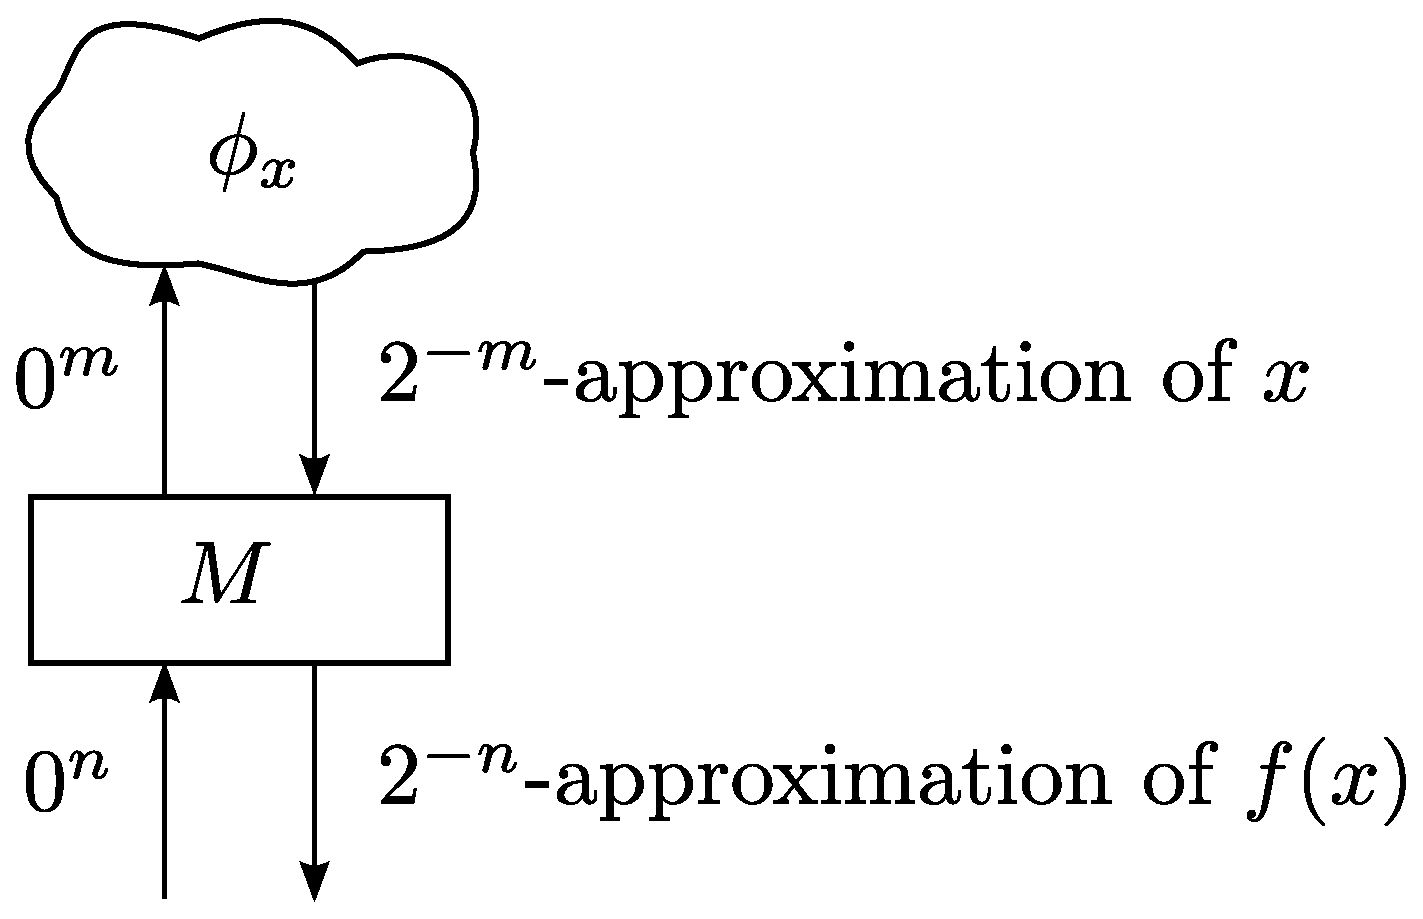
\includegraphics[height=0.15\textheight]{image/model-of-function.eps}
  \end{center}
  \caption{実関数を計算する機械}
 \end{figure}

機械$M$に, 
文字列から文字列への関数$\phi$を神託として与え, 
文字列$0 ^n$を入力として与えたとき, 
出力される文字列を$M ^\phi (0 ^n)$で表す. 
つまり$M ^\phi$をやはり文字列から文字列への関数とみる. 

\begin{definition}
$A$を$\R$の有界閉区間とする. 
神託機械 $M$ が実関数 $f\colon A \to \R$ を計算するとは,
任意の実数 $x \in A$, 任意の $x$ の名 $\phi_x$ にたいして,
$M^{\phi_x}$ が $f(x)$ の名であること.
\end{definition}

$f$が二変数関数であるときには神託を二つ取る機械を考えて同様に定義する. 

 計算可能な実関数は Grzegorczyk によって初めて形式的に定義され,
 \cite{grzegorczyk1955computable}.
 多変数関数のモデルも, 変数と同じ数だけ神託を持つ神託機械によって同様に定義される.

 ある実関数が計算可能であるとは, その関数を計算する神託機械が存在することである.
 同様に, ある実関数が多項式時間計算可能であるとは, その関数を計算する多項式時間神託機械が存在することである.

 神託機械 $M$ がある実関数族 $(f_u)_u$ を計算するとは,
 入力 $u$ を受けったとき, $M_u$ が $f_u$ を計算することである.
 実関数族が多項式時間計算可能であるとは, その実関数族を計算する
 多項式時間神託機械が存在することである.
 

 神託機械 $M$ で $f$ を計算するとき, 求める精度 $n$ にたいして,
 $x$ の近似値に必要な精度 $m$ が定まるため,
 計算可能な関数は連続である.
 また $n$ と $m$ の対応関係と有理数における近似値を与えることで,
 計算可能実関数や多項式時間計算可能実関数にたいして,
 神託機械を用いない同値な特徴付けが可能である.

 \begin{lemma}
  \label{lem:type1representation}
  実関数 $f\colon [0,1] \to \R$ にたいして,
  $\phi_f\colon (\Q \cap [0, 1]) \times \T \to \Q$, $m_f\colon \N \to \N$は
  \begin{align}
   |\phi_f(d, 0^n) - f(d)| \le 2^{-n} 
   &\qquad (d \in (\Q \cap [0,1]), \quad n \in \N)\\
   |x-y| \le 2^{-p_f(m)} \Rightarrow |f(x) - f(y)| \le 2^{-m}
   &\qquad (x, y \in [0, 1], \quad m \in \N)
  \end{align}
 をみたす関数とする.
  \begin{itemize}
   \item $f$ が計算可能であることは, 計算可能な $\phi_f, m_f$ が存在することと同値である. 
   \item $f$ が多項式時間計算可能であることは, 多項式時間計算可能な 
  $\phi_f$, 多項式 $m_f$ が存在することと同値である.
  \end{itemize} 
\end{lemma}

\subsection{困難性}

 関数の下限を示すために, 実関数の計算量クラスに対する困難性を定義する.

 まず実関数の言語に対する還元を定義する.
 言語 $L$ が実関数 $f\colon [0,1] \to \R$ に多項式時間還元可能であるとは,
 $f$ を計算する機械を使って $L(u)$ を多項式時間で計算可能であることである.
 つまり $f$ を計算する機械が与えられ, 入力 $u$ にたいして,
 精度 $n$ を $f$ に与え, ある実数 $x_u$ の神託を模倣し, $f(x_u)$ の $n$ 桁近似値から,
 $u$ が $L$ に含まれるか否かを多項式時間で計算可能であることである
 [図 \ref{fig:reduction}].
 厳密には以下のように定義する.

 \begin{definition}[多項式時間還元可能]
  言語 $L$ が実関数 $f\colon [0,1] \to \R$ に多項式時間還元可能であるとは, 
  任意の文字列 $u$ にたいして, 以下を満たす実数 $x_u \in [0,1]$
  多項式時間計算可能な関数 $R,S,T$ が存在すること.
  \begin{itemize}
   \item $R\colon N \times N \to \{0,1\}, \quad S\colon \N\times \T \to \N, \quad
  T\colon \N \to \T$;
   \item $S(u, \cdot)$ は実数 $x_u$ の名;
   \item 任意の $f(x_u)$ の名 $\phi$ にたいして
	 \[
	  L(u) = R(u, \phi(T(u))).
	 \]
  \end{itemize}
 \end{definition}
 以下単に言語が実関数に還元可能といった場合, 多項式時間還元可能をしめす.
 計算量 $C$ にたいして, 関数 $f$ が $C$困難であるとは,
 任意の $C$ に含まれる言語が $f$ に還元可能であることと定義する.

 \begin{figure}
  \begin{center}
  \label{fig:reduction}
  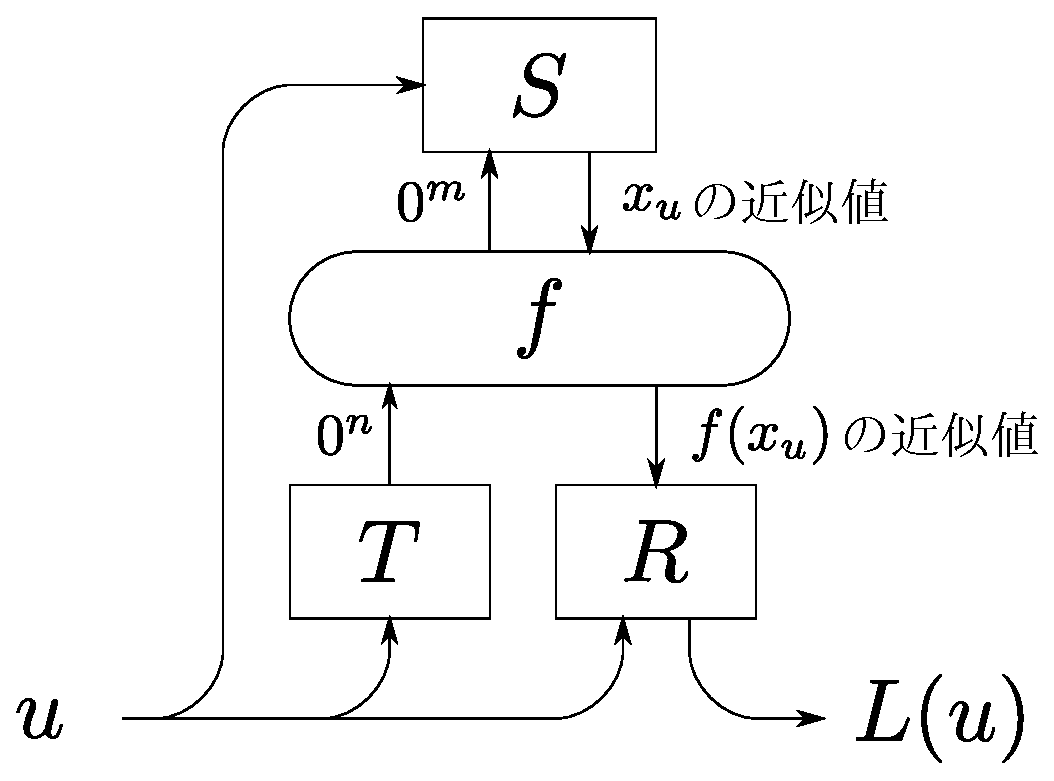
\includegraphics[height=0.2\textheight]{image/reduction.eps}
  \caption{言語 $L$ から関数 $f$ への還元}
  \end{center}
 \end{figure}

 

\section{Proof of The Theorems}
\label{section:differentiable}

We give a proof sketch of Theorem~\ref{DifferentiableIsPspace} and Theorem~\ref{KTimesIsCH}.
First we define a discrete version of differential equations in Section~\ref{section:divp},
and show $\classPSPACE$-hardness or $\classCH$-hardness of the problem with 
restrictions similar to once differentiable or $k$-times differentiable
in Section~\ref{subsection: counting hierarchy}.
In Section~\ref{subsection: ode family}, 
we show that these discrete problems is simulatable
by certain families of smooth differential equations.
We construct the smooth differential equations stated in theorems
putting one family into one real function
in Section~\ref{subsection: proof of theorems}.
Henceforth we call the discrete version of differential equations as difference equations.

The idea to simulate difference equations with differential equations
is essentially from the proof of Lipschitz version \cite{kawamura2010lipschitz}.
In this paper we focus on the structure of difference equations
to analyze precisely the effect of the smoothness restriction.
Consequently we show with the restriction differentiable more than once
differential equations can simulate difference equations whose height is enough small, and it gives the $\classCH$-hardness of smooth differential equations.

\subsection{差分方程式}
\label{section:divp}

この節では微分方程式\eqref{eq:ode}の離散版ともいうべき差分方程式を定義し, 
それが深さの制限に応じて
$\classPSPACE$困難ないし$\classCH$困難であることを示す.

$[n] = \{0, \dots , n-1\}$と書く.
関数$G \colon [P] \times [Q] \times [R] \to \{-1, 0, 1\}$と
$H \colon [P + 1] \times [Q+1] \to [R]$が
任意の$i \in [P]$, $T \in [Q]$について以下を満たすとき(図\ref{fig:divp}), 
\begin{figure}
 \begin{center}
  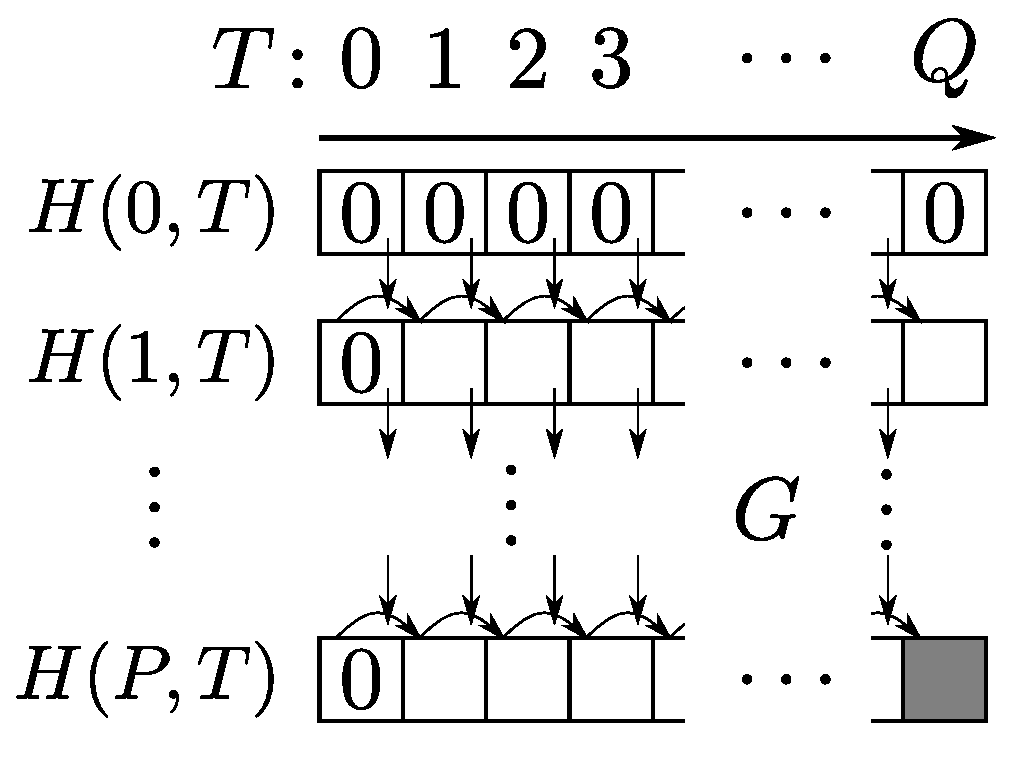
\includegraphics[height=0.15\textheight]{image/divp.eps}
 \end{center}
 \caption{差分方程式$G$とその解$H$}
 \label{fig:divp}
\end{figure}
$H$を\emph{差分方程式}\kern\xkanjiskip$G$の解と呼ぶ.
\begin{gather}
   H(i, 0) = H(0, T) = 0 \label{eq:initial value}
\\
   H(i + 1, T + 1) - H(i+1, T) = G(i, T, H(i, T))  \label{eq:divp}
\end{gather}
$P$, $Q$, $R$をそれぞれこの差分方程式の
\emph{段数}, \emph{列数}, \emph{欄の大きさ}と呼ぶ.
\eqref{eq:ode}の初期条件$h(0) = 0$と方程式$\D h(t) = g(t, h(t))$が
それぞれ式\eqref{eq:initial value}, \eqref{eq:divp}に似ており, 
\ref{subsection: ode family}節ではこれを用いて
微分方程式で差分方程式を模倣する. 


文字列$u$ごとに一つの差分方程式$G _u$を与え,
$u$が言語$L$に属するかをその差分方程式によって計算することを考える.
各 $u$ に対して $G_u$ の段数と列数, 解をそれぞれ $P_u, Q_u, H_u$ としたとき,
言語$L$が関数族$(G_u)_u$によって
\emph{認識}されるとは,
$H_u(P_u, Q_u) = L(u)$ を満たすこととする.

族$(G_u)_u$が\emph{一様}であるとは,
$G_u$の段数, 列数, 欄の大きさそれぞれを$u$を入力とする関数と見做したとき
それらが多項式時間計算可能であり,
かつ与えられた$(u, i, T, Y)$から多項式時間で$G_u(i, T, Y)$が
計算できることと定義する.
そのようなとき$G _u$の段数, 列数及び欄の大きさは,
$|u|$の多項式の指数($2^{\mathrm{poly} (|u|)}$)で抑えられる.
$G_u$の段数を$P_u$と置くとき, 多項式$p$が存在して$P_u \le p(|u|)$が成立つとき,
族 $(G_u) _u$は\emph{多項式段}であるという.
また定数$c,d$が存在して$P_u \le c \log(|u|)+d$が成立つとき,
族 $(G_u) _u$は\emph{対数段}であるという. 
この用語を使うと, 
河村がLipschitz連続な場合の解析に用いた補題
\cite[補題4.7]{kawamura2010lipschitz}は次のように書ける. 

\begin{lemma}
 \label{DIVPpolyIsPSPACEhard}
 多項式段の一様な差分方程式族によって認識される$\classPSPACE$困難な言語が存在する
 \footnote{差分方程式によって認識される言語のクラスはカープ帰着において閉じており,
多項式段一様な関数族によって認識される言語は$\classPSPACE$と一致する.}.
\end{lemma}

河村\cite{kawamura2010lipschitz}は
この多項式段の一様な差分方程式族をLipschitz連続な微分方程式で模倣することで, 
表\ref{table:related}第三行の結果を得た. 
本稿の定理\ref{DifferentiableIsPspace}はこの構成に手を加えて, 
$(\infty, 1)$回微分可能な模倣に
作り替えることにより
(\ref{subsection: ode family}, \ref{subsection: proof of theorems}節), 
やはり補題\ref{DIVPpolyIsPSPACEhard}から得られる. 

本稿では更に, 対象とする差分方程式族を対数段に制限すれば, 
$(\infty, 2)$回以上微分可能な関数によっても
模倣できることを示し
(\ref{subsection: ode family}, \ref{subsection: proof of theorems}節), 
これと次の補題から定理\ref{KTimesIsCH}を得る. 

\begin{lemma}
 \label{DIVPlogIsCHhard}
 対数段の一様な差分方程式族によって認識される$\classCH$困難な言語が存在する.
\end{lemma}

計数階層$\classCH$の定義と差分方程式の関係及び
補題\ref{DIVPlogIsCHhard}の証明は
\ref{subsection: counting hierarchy}節にて述べる.


\subsection{The Counting Hierarchy and Difference Equations of Logarithmic Height}
\label{subsection: counting hierarchy}

The polynomial hierarchy~$\classPH$ is defined using non-deterministic polynomial-time oracle Turing machines: 
\begin{align}
 \classSigma^p_0  &= \classP,
 &
 \classSigma^p_{n+1} &= \classNP ^{\classSigma^p_n},
 &
 \classPH &= \bigcup_n \classSigma^p_n.
\end{align}
In the same way, the counting hierarchy~$\classCH$
\cite{wagner1986complexity} 
is defined
using probabilistic polynomial-time oracle Turing machines%
\footnote{This characterization, introduced by Tor{\'a}n 
in \cite{toran1991complexity}, is different from Wagner's original one.
}: 
\begin{align} \label{eq:CH}
 \quantC_0 \classP  &= \classP,
 &
 \quantC_{n+1} \classP &= \classPP^{\quantC_n \classP},
 &
 \classCH &= \bigcup_n \quantC_n \classP.
\end{align}
It is known that $\classPH \subseteq \classCH \subseteq \classPSPACE$, 
but we do not know whether $\classPH = \classPSPACE$.


Each level of the counting hierarchy 
has a complete problem defined as follows.
For every formula $\phi(X)$ with the list $X$ of $l$ free propositional variables,
we write 
\begin{equation}
 \quantC^m X \phi(X) 
  \longleftrightarrow 
  \sum_{X \in \{0,1\}^l} \phi(X) \ge m,
\end{equation}
where $\phi(X)$ is identified with the function 
$\phi \colon \{0,1\}^l \to \{0,1\}$
such that $\phi(X) = 1$ if and only if $\phi(X)$ is true.
This ``counting quantifier'' $\quantC ^m$ generalizes 
the usual quantifiers $\exists$ and $\forall$, 
because $\quantC^1 = \exists$ and $\quantC^{2^l} = \forall$.
For lists $X _1$, ldots, $X _n$ of variables 
and a formula $\phi(X_1, \dots, X_n)$ with all free variables listed, 
we define
\begin{equation}
 \langle \phi(X_1, \dots, X_n), m_1, \dots, m_n \rangle \in \quantC_n B_{be}
 \longleftrightarrow
 \quantC^{m_1}{X_1} \cdots \quantC^{m_n}{X_n} \phi(X_1, \dots, X_n).
\end{equation}

\begin{lemma}[{\cite[Theorem 7]{wagner1986complexity}}] \label{lemma:CnP-complete}
 For every $n \ge 1$, 
 the problem $\quantC_n B_{be}$ is $\quantC_n\classP$-complete.
\end{lemma}

We define a problem $\quantC_{\log} B_{be}$ by
\begin{equation}
 \langle 0^{2^n}, u \rangle \in \quantC_{\log} B_{be}
 \longleftrightarrow
 u \in \quantC_n B_{be}.
\end{equation}
We show that $\quantC_{\log} B_{be}$ 
is $\classCH$-hard and recognized by a logarithmic-height uniform function family,
as required in Lemma~\ref{DIVPlogIsCHhard}. 

\begin{proof}[\textup{Proof of Lemma~\ref{DIVPlogIsCHhard}}]
First we prove that $\quantC_{\log} B_{be}$ is $\classCH$-hard.
For each problem $A$ in $\classCH$, there is a constant $n$ such that $A \in \quantC_n \classP$.
From Lemma~\ref{lemma:CnP-complete}, for each $u \in \{0,1\}^*$
there is a polynomial-time function $f_n$ such that
$u \in A \leftrightarrow f_n(u) \in \quantC_n B_{be}$. So
\begin{align}
 u \in A 
 & \longleftrightarrow \langle 0^{2^n}, f_n(u) \rangle \in \quantC_{\log} B_{be}.
\end{align}
Since $\langle 0^{2^n}, f_n(\cdot) \rangle$ is polynomial time computable,
$A$ is reducible to $\quantC_{\log} B_{be}$.


Next we construct a logarithmic-height uniform function family $(G_u)_u$
recognizing $\quantC_{\log} B_{be}$.
Let $u  = \langle 0^{2^n}, 
\langle \phi(X_1, \dots, X_n), m_1, \dots, m_n \rangle \rangle$, 
where $n$, $m_1, \dots, m_n$ are nonnegative integers 
and $\phi$ is a formula. 
(If $u$ is not of this form, then $u \notin \quantC_{\log} B_{be}$.)
 
We write $l_i = |X_i|$ and $s_i = i + \sum^i_{j=1}l_j$.
For each $i \in \{0, \dots, n\}$ and
$Y_{i+1} \in \{0,1\}^{l_{i+1}}, \dots, Y_n \in \{0,1\}^{l_n}$,
we write $\phi_i(Y_{i+1}, \dots, Y_n)$ for the truth value of the subformula
$\quantC^{m_{i}}{X_i} \cdots \quantC^{m_1}{X_1} \phi(X_1, \dots, X_i, Y_{i+1}, \dots, Y_n)$,
so that $\phi_0 = \phi$ and $\phi_n() = \quantC_{\log} B_{be} (u)$.
We regard the quantifier $\quantC^m$ as a function from $\N$ to $\{0,1\}$:
\begin{equation}
 C^m(x) 
  = \begin{cases}
     1 & \text{if} \ x \ge m, \\
     0 & \text{if} \ x < m.
    \end{cases}
\end{equation}
Thus,
\begin{equation} \label{eq:phi-step}
 \phi_{i+1}(Y_{i+2}, \dots, Y_n) 
  = C^{m_{i+1}}\left(\sum_{X_{i+1} \in \{ 0,1 \} ^{l_i}}
		\phi_i(X_{i+1}, Y_{i+2}, \dots, Y_{n})\right).
\end{equation}
For $T \in \N$, we write $T_i$ for the $i$th digit of $T$ written in binary,
and $T_{[i,j]}$ for the string $T_{j-1} T_{j-2} \cdots T_{i+1} T_{i}$.

For each $(i, T, Y) \in [n+1] \times [2^{s_n}+1] \times [2^{|u|}]$,
we define $G_u (i, T, Y)$ as follows.
The first row is given by
 \begin{equation}\label{eq:def-Gu:case0}
  G_u(0,T,Y) = 
   (-1)^{T_{s_1}}\phi(T_{[1,s_1]}, T_{[s_1+1,s_2]},
    \dots, T_{[s_{n-1}+1,s_n]}), 
 \end{equation}
and for $i \neq 0$, we define 
 \begin{equation} 
  G_u(i,T,Y) = 
   \begin{cases}
    (-1)^{T_{s_{i+1}}} C^{m_i}(Y) 
    & \text{if} \ T_{[1,s_i+1]} = 10 \cdots 0, \\
    0 & \text{otherwise}.
   \end{cases} 
 \end{equation}
Define $H_u$ from $G_u$ by \eqref{eq:initial value} and \eqref{eq:divp}.

We prove by induction on $i$ that $H_u(i, T) \in [2^{l_u}]$ for all $T$, and that
 \begin{equation} \label{eq:subformula}
  G_u(i,T,H_u(i,V)) = (-1)^{V_{s_{i+1}}} 
   \phi_i(V_{[s_i+1, s_{i+1}]}, \dots, V_{[s_{n-1}+1, s_n]})
 \end{equation}
for all $i \in [n+1]$ and $V \in [2^{s_n}+1]$
such that $V_{[1, s_i +1]} = 10 \cdots 0$.

For $i=0$, the claims follows from \eqref{eq:def-Gu:case0}.
For the induction step, assume \eqref{eq:subformula}. 
We have
 \begin{equation} \label{eq:summation}
  H_u(i+1, T) 
  = \sum_{V = 0}^{T-1} G_u(i, V, H_u(i, V)) 
  = \sum_{V} (-1)^{V_{s_{i+1}}} \phi_i(V_{[s_i+1, s_{i+1}]}, 
   \dots, V_{[s_{n-1}+1, s_n]}),
 \end{equation}
where we write $\overline U$ for the number represented by string $U$ as binary expression.
For each $V < \overline{T_{[s_{i+1}+1, s_n]} 0 \cdots 0}$ in \eqref{eq:summation},
the term $\phi_i(V_{[s_i+1, s_{i+1}]}, \dots, V_{[s_{n-1}+1, s_n]})$ and
 $- \phi_i(V_{[s_i+1, s_{i+1}]}, \dots, V_{[s_{n-1}+1, s_n]}) = 0$ cancel each other out. Then 
 \begin{equation}
  H_u(i+1, T) = \sum_{X \in \{0,1\}^{l_i}}
  \phi_i(X, T_{[s_{i+1}+1, s_{i+2}]}, \dots, T_{[s_{n-1}+1, s_n]}).
 \end{equation}
 From this equation and \eqref{eq:phi-step}, it follows that
 \begin{align}
  G_u(i+1,T,H_u(i+1,T)) 
  &= (-1)^{T_{s_{i+2}}} C^{m_{i+1}} (H_u(i+1, T))
\notag
\\
  &= (-1)^{T_{s_{i+2}}} \phi_{i+1}(T_{[s_{i+1}+1, s_{i+2}]}, \dots, T_{[s_{n-1}+1, s_n]}).
 \end{align}


By substituting $n$ for $i$ and $2^{s_n}$ for $T$ in \eqref{eq:subformula},
we get $G_u(n, 2^{s_n}, H_u(n,2^{s_n})) = \phi_n() = \quantC_{\log} B_{be}(u)$.
Hence $H_u(n+1, 2^{s_n}+1) = \quantC_{\log} B_{be}(u)$.
 
The height $n+1$, the width $2^{s_n}+1$, and the cell size $2^{|u|}$
of $G_u$ are polynomial-time computable from $u$, 
and $n+1 \le \log(|0^{2^n}|) + 1 \le \log|u| + 1$.
Hence $(G_u)_u$ is uniform and has logarithmic height. 
\end{proof}


The language class recognized by uniform function families with $i$ rows
contains $\quantC_i \classP$ (the $i$th level of the counting hierarchy)
and is contained in $\quantC_{i+1} \classP$.
While the class $\quantC_i \classP$ is defined by \eqref{eq:CH} using oracle Turing machines,
it is also characterized as those languages Karp-reducible to $\quantC_i B_{be}$, or 
as those accepted by a polynomial-time alternating Turing machine 
extended with ``threshold states'' and having at most $i$ alternations.
Likewise, 
the language class accepted by uniform function families of logarithmic height
coincided with languages Karp-reducible to $\quantC_{\log} B_{be}$
and with those accepted by an extended alternating Turing machine with logarithmic alternations.
Since this class contains $\classCH$,
we only state $\classCH$-hard in Lemma~\ref{KTimesFamily} and Theorem $\ref{KTimesIsCH}$,
but it is not known such class how hard the class is between $\classCH$ and $\classPSPACE$.



\subsection{Families of Real Functions Simulating Difference Equations}
\label{subsection: ode family}
We show that families of smooth differential equations can simulate 
$\classPSPACE$-hard or $\classCH$-hard difference equations stated in previous section.

Before stating Lemma~\ref{KTimesFamily} and Lemma~\ref{DifferentiableFamily},
we extend the definition of polynomial-time computability of real function
to families of real functions.
A machine $M$ \emph{computes} a family $(f_u)_u$ of functions $f _u \colon A \to \R$ 
indexed by strings $u$
if for any $x \in A$ and any name $\phi_x$ of $x$,
the function taking $v$ to $M ^{\phi _x} (u, v)$ is a name of $f _u (x)$.
We say a family of real functions $(f_u)_u$ is polynomial-time if there is
a polynomial-time machine computing $(f_u)_u$.

 \begin{lemma}
  \label{KTimesFamily}
  There exist a $\classCH$-hard language $L$ and a polynomial $\mu$ 
  such that for all $k \ge 1$ and polynomials $\gamma$,
  there are a polynomial $\rho$ and families $(g_u)_u$, $(h_u)_u$ of real functions
  having following properties that $(g_u)_u$ is polynomial-time computable and for any string $u$:
  \begin{enumerate}
   \item \label{enum:kf:start}
	 $g_u\colon [0,1] \times [-1,1]\to \R$, $h_u\colon [0,1] \to [-1,1]$;
   \item \label{enum:equation}
	 $h_u(0) = 0$ and $\D h_u(t) = g_u(t, h_u(t))$ for all $t \in [0,1]$;
   \item \label{enum:differentiability}
         $g_u$ is $(\infty, k)$-times continuously differentiable;
   \item \label{enum:boundary}
	 $
	 \D^{(i, 0)} g_u(0,y) = \D^{(i, 0)} g_u(1,y) = 0
         $ for all $i \in \N$ and $y \in [-1,1]$;
   \item \label{enum:smooth}
	 $
	 \left|\D^{(i,j)} g_u(t,y)\right| \le 2^{\mu(i, |u|) - \gamma(|u|)}
         $ for all $i \in \N$ and $j \in \{0, \dots, k\}$;
   \item \label{enum:kf:end}
	 $h_u(1) = 2^{-\rho(|u|)} L(u)$.
  \end{enumerate}
 \end{lemma}

\begin{lemma}
 \label{DifferentiableFamily}
 There exist a $\classPSPACE$-hard language $L$ and a polynomial $\mu$,
 such that for all polynomials $\gamma$,
 there are a polynomial $\rho$ and families $(g_u)_u$, $(h_u)_u$ of real functions
 such that $(g_u)_u$ is polynomial-time computable and for any string $u$
 satisfying (\ref{enum:kf:start})--(\ref{enum:kf:end}) of Lemma~\ref{KTimesFamily} with $k = 1$.
\end{lemma}

We will prove Lemma~\ref{KTimesFamily} using Lemma~\ref{DIVPlogIsCHhard} as follows.
Let a function family $(G_u)_u$ be as in Lemma~\ref{DIVPlogIsCHhard},
and let $(H_u)_u$ be the solution of the difference equation given by $(G_u)_u$.
We construct $h_u$ and $g_u$ from $H_u$ and $G_u$ 
such that $h_u(T/2^{q(|u|)}) = \sum^{p(|u|)}_{i = 0} H_u(i, T)/B^{d_u(i)}$ for each $T = 0$, \ldots, $2^{q(|u|)}$
and $\D h_u(t) = g_u(t, h_u(t))$.
The polynomial-time computability of $(g_u)_u$ follows from that of $(G_u)_u$.
We can prove Lemma~\ref{DifferentiableFamily} from Lemma~\ref{DIVPpolyIsPSPACEhard} in the same way.

In Lemma~\ref{KTimesFamily}, 
we have the new conditions (\ref{enum:differentiability})--(\ref{enum:smooth}) 
about the smoothness and the derivatives of $g_u$ 
that were not present in \cite[Lemma 4.1]{kawamura2010lipschitz}.
To satisfy these conditions, we construct $g_u$ 
using the smooth function $f$ in following lemma.

\begin{lemma}[{\cite[Lemma 3.6]{ko1991complexity}}]
 \label{SmoothFunction}
 There exist a polynomial-time infinitely differentiable function  $f \colon [0,1] \to \R$ 
 and a polynomial $s$ such that
  \begin{enumerate}
   \item $f(0) = 0$ and $f(1) = 1$;
   \item $\D ^n f (0) = \D ^n f (1) = 0$ for all $n \ge 1$;
   \item $f$ is strictly increasing;
   \item $\D ^n f$ is polynomial-time computable for all $n \ge 1$;
   \item \label{enum:polynomial-size}
	 $|\D^n f| \le s(n)$ for all $n \ge 1$. 
  \end{enumerate}
 \end{lemma}

Although the existence of the polynomial~$s$ satisfying the condition (\ref{enum:polynomial-size}) is not stated in \cite[Lemma 3.6]{ko1991complexity},
it can be shown easily.

We only prove Lemma~\ref{KTimesFamily} here
and omit the analogous and easier proof of Lemma~\ref{DifferentiableFamily}.

\begin{proof}[Proof of Lemma~\ref{KTimesFamily}]
Let a function family $(G_u)_u$ be as in Lemma~\ref{DIVPlogIsCHhard},
and let a function family $(H_u)_u$ be the solution of the difference equation given by $(G_u)_u$.

By a similar argument to the beginning of the proof\cite[Lemma 4.1]{kawamura2010lipschitz},
we may assume that there exist polynomial-time functions $p$, $j_u$
and polynomial $q$, $r$ satisfying following properties:
\begin{gather}
 G_u \colon [p(|u|)] \times [2^{q(|u|)}] \times [2^{r(|u|)}] \to \{-1, 0, 1\};
 \\
 H_u(i, 2^{q(|u|)}) = \begin{cases}
		       L(u) & (i=p(|u|)) \\
		       0 & (i<p(|u|))
		      \end{cases};
 \\
 i \not = j_u(T)  \to G_u(i, T, Y) = 0.
\end{gather}
Since $G_u$ has logarithmic height,
there exists polynomial $\sigma$ such that $(k+1)^{p(x)} \le \sigma(x)$


We construct the families real functions $(g_u)_u$ and $(h_u)_u$ simulating $G _u$ and $H _u$,
in particular, $h_u(T/2^{q(|u|)}) = \sum^{p(|u|)}_{i = 0}H_u(i, T)/B^{d_u(i)}$.
We define the constant $B$ and the function $d_u \colon [p(|u|)+1] \to \N$ as
  \begin{align}
   B &= 2^{\gamma(|u|) + r(|u|) + s(k) + k + 3}
   &
   d_u(i) &= 
   \begin{cases}
    \sigma(|u|) & (i=p(|u|)) 
    \\
    (k+1)^i & (i<p(|u|)).
   \end{cases}
  \end{align}
For each $(t, y) \in [0,1] \times [-1, 1]$,
there exists unique $N \in \N$, $\theta \in [0,1)$, $Y \in \Z$ and $\eta \in [-1/4, 3/4)$
such that $t = (T + \theta)2^{-q(|u|)}$ and $y = (Y + \eta)B^{-d_u(j_u(T))}$.
Let $f$ and a polynomial $s$ be as in Lemma~\ref{SmoothFunction},
we define 
$\delta_{u,Y} \colon [0,1] \to \R$,
$
g _u \colon [0, 1] \times [-1, 1] \to \R
$ and $
h _u \colon [0, 1] \to [-1, 1]
$ as
  \begin{align}
    \label{eq:delta}
   \delta_{u, Y} (t) &= \frac{2^{q(|u|)} \D f(\theta)}{B^{d_u(j_u(T)+1)}} 
   G_u \bigl( j_u(T), T, Y \bmod 2^{r(|u|)} \bigr),
   \\
  \label{eq:gu}
  g_u(t,y) 
  &= \begin{cases}
     \delta_{u, Y}(t)
     & (\eta \le \frac 1 4)
     \\
     ( 1-f ( \frac{4\eta-1}{2})) \delta_{u, Y}(t)
     + f ( \frac{4\eta-1}{2}) \delta_{u,Y+1}(t)
     & (\eta > \frac 1 4),
    \end{cases}
   \\
  h_u(t) 
   &= \sum^{p(|u|)}_{i=0} \frac{H_u(i, T)}{B^{d_u(i)}}  
  + \frac{f(\theta)}{B^{d_u(j_u(T)+1)}} G_u \bigl( j_u(T), T, H_u(j_u(T), T) \bigr) .
  \label{eq:hu}
  \end{align}

We will verify that $(g_u)_u$ and $(h_u)_u$ defined above satisfy all the conditions stated in Lemma~\ref{KTimesFamily}.
The condition(\ref{enum:equation}) are verified by applying the same argument of
\cite[Lemma 4.1]{kawamura2010lipschitz}.

We will show that the condition(\ref{enum:differentiability}) holds, that is, $g _u$ is $(\infty, k)$-times continuously differentiable.
For each $i \in \N$,
  \begin{align}
   \D^i \delta_{u,Y}(t) 
&
    = \frac{2^{(i+1)q(|u|)} \D^{i+1}f(\theta)}{B^{d_u(j_u(T)+1)}}
    G_u\left( j_u(T),\ T,\ Y \bmod 2^{r(|u|)} \right),
\\
   \label{eq:derivativeofgu}
    \D^{(i,0)} g_u(t, y)
&
     = \begin{cases}
 	\D^i \delta_{u, Y}(t) 
	& (- \frac 1 4 < \eta < \frac 1 4) \\
	\left( 1-f \left(\frac{4\eta-1}{2}\right)\right) 
	\D^i \delta_{u, Y}(t)
	+ f \left(\frac{4\eta-1}{2}\right) \D^i \delta_{u,Y+1}(t) 
	& (\frac 1 4 < \eta < \frac 3 4),
       \end{cases}
  \end{align}
and for each  $j \in \{1, \dots , k\}$,
  \begin{equation}
    \D^{(i,j)} g_u(t, y)
     = \begin{cases}
	0 & (- \frac 1 4 < \eta < \frac 1 4) \\
	(2B^{d_u(j_u(T))})^j \D^j f(\frac{4\eta - 1}2)
	(\D^i \delta_{u,Y+1}(t)-\D^i \delta_{u, Y}(t)) 
	& (\frac 1 4 < \eta < \frac 3 4).
       \end{cases}
  \end{equation}
It is easy to check that they are also continuous on boundaries($\theta = 0$, $\eta = -1/4, 3/4$).
Hence $g _u$ is $(\infty, j)$-times continuously differentiable.
Substituting $t = 0, 1$ ($\theta = 0$) into \eqref{eq:derivativeofgu},
we get $\D^{(i, 0)} g_u(0,y) = \D^{(i, 0)} g_u(1,y) = 0$, 
so the condition (\ref{enum:boundary}) holds.

We show that the condition (\ref{enum:smooth}) holds with $\mu(x, y) = (x+1)q(y) + s(x+1)$.
Note that $\mu$ is a polynomial independent from $k$ or $\gamma$.
Since $|\D^i \delta_{u,Y}(t)| \le 2^{(i+1)q(|u|) + s(i+1)}B^{-d_u(j_u(|u|)+1)}$ by \eqref{eq:delta}, for all $i \in \N$ and $j \in \{0, \dots, k\}$,
 \begin{equation}
  |\D^{(i,j)} g_u| 
   \le 
   2^k B^{k \cdot j_u(T)} 2^{s(k)} \cdot 2 \cdot 
   \frac{2^{(i+1)q(|u|) + s(i+1)}}{B^{d_u(j_u(|u|)+1)}} 
   \le
   \frac{2^{\mu(i, |u|) + s(k) + k + 1}}{B}
   \le
   2^{\mu(i, |u|) - \gamma(|u|)}
 \end{equation}
 by our choice of $B$.

We have (\ref{enum:kf:end}) with
  $\rho(x) = \sigma(x) \cdot (\gamma(x)+r(x)+s(k)+k+3)$ because
  \begin{equation}
   h_u(1) = \frac{H_u(p(|u|), 2^{q(|u|)})}{B^{d_u(p(|u|))}} 
          = \frac{L(u)}{2^{\sigma(|u|) \cdot (\gamma(|u|)+r(|u|)+s(k)+k+3)}}
	  = 2^{-\rho(|u|)} L(u).
  \end{equation}
 \end{proof}



 To prove Lemma~\ref{DifferentiableFamily}, 
 let a function family $(G_u)_u$ be as Lemma~\ref{DIVPpolyIsPSPACEhard}
 and a function family $(H_u)_u$ be the solution of the difference equation given by $(G_u)_u$,
 and define $(g_u)_u$ and $(h_u)_u$ as \eqref{eq:gu} and \eqref{eq:hu}
 with $d_u(i) = i$.
 It is shown in the same way above that they match all the conditions
 stated in Lemma~\ref{DifferentiableFamily}.


\subsection{The Proof of Main Theorems}
\label{subsection: proof of theorems}
We describe the sketch of proof.
Let $(g_u)_u$ and $(h_u)_u$ be as lemmas in the previous section,
the real functions $g$ and $h$ in theorems are constructed from $(g_u)_u$ and $(h_u)_u$ as follows.
Divide $[0,1)$ into infinity many subintervals $[l^-_u, l^+_u]$,
with midpoints $c_u$.
We construct $h$ putting a scaled copy of $h_u$ onto $[l^-_u, c_u]$ and
putting a horizontally reversed scaled copy of $h_u(t)$ onto $[c_u, l^+_u]$ 
so that $h(l^-_u) = 0$, $h(c_u) = 2^{-\rho'(|u|)} L(u)$ and $h(l^+_u) = 0$ where $\rho'$ is a polynomial.
In the same way, $g$ is constructed from $(g_u)_u$ so that $g$ and $h$ satisfy \eqref{eq:ode}.

We omit the proof of Theorem~\ref{DifferentiableIsPspace} 
since we can get it applying the same argument as the proof of Theorem~\ref{KTimesIsCH} and using Lemma~\ref{DifferentiableFamily}.


\begin{proof}[Proof of Theorem~\ref{KTimesIsCH}]
Let $L$ and $\mu$ be as Lemma~\ref{DifferentiableFamily}.
Define
 \begin{align}
  \lambda(x) &= 2x + 2,&
  \gamma(x) &= x \mu(x, x) + x \lambda(x).
 \end{align}
and for each $u$
\begin{align}
 \Lambda_u 
 &= 2^{\lambda(|u|)}, &
 c_u 
 &= 1-\frac{1}{2^{|u|}}+\frac{2\bar{u}+1}{\Lambda_u}, &
 l_u^\mp 
 &= c_u\mp\frac{1}{\Lambda_u}
\end{align}  
 where $\bar u \in \{0, \dots, 2^{|u|} - 1\}$ is the number represented by $u$ as binary expression.
Let $\rho$, $(g_u)_u$, $(h_u)_u$ be as Lemma~\ref{KTimesFamily} with $\gamma$.

We define
 \begin{align} \label{eq:g}
 g \left(l^\mp_u \pm \frac{t}{\Lambda_u}, \frac{y}{\Lambda_u}\right)
  &= \begin{cases}
      \pm \displaystyle \sum_{l=0}^k \frac{\D^{(0,l)}g_u(t,1)}{l!} (y-1)^l 
      &  (1<y) \\
      \pm g_u(t, y)      & (-1 \le y \le 1) \\
      \pm \displaystyle \sum_{l=0}^k \frac{\D^{(0,l)}g_u(t,-1)}{l!} (y+1)^l  
      &  (1<y) \\
    \end{cases} 
  \\
 h \left( l^\mp_u \pm \frac{t}{\Lambda_u} \right) 
  & = \frac{h_u(t)}{\Lambda_u}
\end{align}
for each string $u$, $t \in [0,1)$, $y \in [-1, 1]$.
Let $g(1,y) = 0$ and $h(1) = 0$ for any $y \in [-1,1]$

It can be shown in a similar way as the Lipschitz version 
that $g$ and $h$ satisfy \eqref{eq:ode} and $g$ is polynomial-time computable,
so see the proof of \cite[Theorem 3.2]{kawamura2010lipschitz} for more details.
We only show that $g$ is $(\infty, k)$-times continuously differentiable.

For each $i \in \N$ and $j \in \{0, \dots, k\}$ differentiating \eqref{eq:g} $(i,j)$-times,
\begin{equation}
   \D^{(i, j)}g \left(l^\mp_u \pm \frac{t}{\Lambda_u}, \frac{y}{\Lambda_u}\right)
   = \begin{cases}
      \pm \Lambda_u^{(i, j)} \sum^{k}_{l=j} \frac{\D^{(i,l)} g_u(t,1)}{(l-j)!}
      (y - 1)^l &  (1<y)
      \\
      \pm \Lambda_u^{(i,j)} \D^{(i, j)} g_u(t, y) & (-1 < y < 1)
      \\
      \pm \Lambda_u^{(i, j)} \sum^{k}_{l=j} 
      \frac{\D^{(i,l)} g_u(t, -1)}{(l-j)!} (y + 1)^l &  (1<y).
    \end{cases}
\end{equation}
for $t \in (0, 1)$ and $y \in [-\Lambda_u, \Lambda_u]$ where $y \neq -1, 1$.
It is continuous where $t \in (0,1)$ and $y \not = -1, 1$
since each $\D^{(i,j)}g_u$ is continuous.
We can verify that it is continuous on the boundary($t = 0, 1$ or $y = -1, 1$)
by the definition and Lemma~\ref{KTimesFamily} (\ref{enum:boundary}).
Finally we show that it is continuous at 1 for the first variable.
By Lemma~\ref{KTimesFamily} (\ref{enum:smooth}),
 \begin{align}
  \left|\D^{(i, j)}g \left(l^\mp_u \pm \frac{t}{\Lambda_u},
  \frac{y}{\Lambda_u}\right)\right|
  &\le 
  \Lambda_u^{i+j} \sum^{k}_{l=j} |\D^{(i,l)} g_u | (\Lambda_u + 1)^l 
  \notag
  \\
  & \le \Lambda_u^{i+j+k}  2^{k + \mu(i, |u|) - \gamma(|u|)}
   =  2^{(i+j+k)\lambda(|u|) + k + \mu(i, |u|)  - \gamma(|u|)}. 
  \label{eq:sizeofderivative}
 \end{align}
While $|u| \to \infty$, \eqref{eq:sizeofderivative} correspondingly approaches to $0$ by our choice of $\gamma$.
Hence $\lim_{t \to 1-0}\D^{(i,j)} g(t,y) = g(1, y) = 0$.
and we complete to show that $g$ is $(\infty, k)$-times continuously differentiable.
\end{proof}



\section{演算子の計算量}

Both Theorem~\ref{DifferentiableIsPspace} and \ref{KTimesIsCH}
states the complexity of the solution $h$ under the assumption 
that $g$ is polynomial-time computable.
How complex can it be to ``solve'' differential equations,
i.e., how complex is the operator computing $h$ by given $g$?
To make an answer to this problem,
we need to define complexity of operators from real functions to real functions.

To discuss complexity of real functions,
we encode real numbers by functions from string to string.
We use string functions as names of elements in $\R$,
such relation is called representation of $\R$.
In the same way, we represent real functions as string functions
to discuss complexity of real operators.
So we need to define representations as string functions of
class $\classC_{[0, 1]}$ of continuous real functions $h \colon [0,1] \to \R$ 
and class $\classLip_{[0, 1] \times [-1, 1]}$ of Lipschitz continuous real functions.
The choice of representations is important since the computability and complexity is depending on these representations.
Following \cite{kawamura2010operators},
we use $\deltabox$ as the representation of $\classC_{[0,1]}$ and $\deltaboxLip$ as the representation of $\classLip_{[0, 1] \times [-1, 1]}$.
It is known that is some sense $\deltabox$ an unique natural representation of $\classC_{[0, 1]}$ \cite{kawamura11:_funct_space_repres_and_polyn_time_comput}.
And $\deltaboxLip$ is a representation
added information about the Lipschitz constant to $\deltabox$.

Since size of string functions are not finite,
by restricting the amount of resources (time and space) of oracle Turing machine using second order polynomial,
we define second-order complexity classes
(e.g. $\classFPSPACEtwo$, polynomial-space computable),
reductions (e.g. $\redW$, polynomial-time Weihrauch reduction),
and hardness.
Combining it with the representations of real functions described above,
we can write theorems of this paper in constructive form.

Let $\OpIVP$ be an operator mapping a real function $g$ of class $\classLip_{[0, 1] \times [-1, 1]}$ to
the solution $h$ of \eqref{eq:ode} of class $\classC_{[0, 1]}$.
The operator $\OpIVP$ is a partial projection from $\classLip [[0, 1] \times [-1, 1]]$ to $\classC [0, 1]$.
\cite[定理4.9]{kawamura2010operators}では表\ref{table:related}第三行の証明を
構成的に書き直すことで, 
$\OpIVP$が$(\deltaboxLip, \deltabox)$-$\classFPSPACEtwo$-$\redW$完全であることが
示された. 
本稿の定理\ref{DifferentiableIsPspace}も同じように
構成的に書き直すことができる. 
即ち$\OpIVP$を$(\infty, k)$回連続微分可能な入力に制限したものを
$\OpIVP _k$と書くと, 

\begin{theorem}
\label{theorem: C1 constructive}
$\OpIVP _1$は$(\deltaboxLip, \deltabox)$-$\classFPSPACEtwo$-$\redW$完全. 
\end{theorem}

これを示すには, 
定理\ref{DifferentiableIsPspace}の証明において
関数の構成に使われた情報が入力から容易に得られることを確かめればよく, 
新たな技巧を要しないから詳細は省略する. 
この構成的な主張は非構成的な主張よりも
強いものであり\cite[補題3.7, 3.8]{kawamura2010operators}, 
定理\ref{DifferentiableIsPspace}は
定理\ref{theorem: C1 constructive}の系として従う. 

% \begin{theorem}
% \label{theorem: Ck constructive}
% \end{theorem}

なお定理\ref{KTimesIsCH}も同様に構成的な形で成立ち, 
各$k \in \N$について
$\OpIVP _k$は$(\deltaboxLip, \deltabox)$-$\classCHtwo$-$\redW$困難であるが, 
この\cite{kawamura2010operators}の枠組における$\classCHtwo$を定義するには
相対化の扱いについて今少しの議論を要するので別稿で扱う. 

% ところで, より強い帰着である
% 強ワイラオホ帰着を用いると

% \begin{theorem}
% $\OpIVP _\infty$は$(\deltaboxLip, \deltabox)$-$\classFPSPACEtwo$-$\redSW$完全. 
% \end{theorem}

\section{今後の課題}
1つ目の課題は$(\infty, k)$回連続微分可能という制限の元でのタイトな計算量を見つけることである.
定理$\ref{KTimesIsCH}$では便宜上$\classCH$困難と述べるに留まっているが,
少なくとも\ref{subsection: counting hierarchy}節において定義した
$\quantC_{\log} B_{be}$にカープ帰着可能な言語のクラスについて困難であることは示せる.
%また交替性機械を計数階層を特徴付けるに拡張したとき, 交替回数が入力の対数オーダーで抑えられる機械によって受理される言語クラスと一致する.
そのようなクラスが$\classCH$と$\classPSPACE$の間のどこに位置するかは以前不明である.

2つ目の課題は$g$について任意回連続微分可能と解析的の間の制限と
常微分方程式の解の計算量の変化の関係の解明である.
特に無限回微分可能性と計算量の下限の関係については, 他の問題に関して
いくつかの否定的な結果があるが, 常微分方程式においてはどう変化するのか.

また前節でも述べたとおり, 構成的な形での定理 \ref{KTimesIsCH} については別稿にて扱う.

\section*{謝辞}

本研究を遂行し発表するにあたり
日本学術振興会「組織的な若手研究者等海外派遣プログラム」及び
文部科学省科学研究費補助金若手研究(B)\,23700009による援助を受けた. 
記して謝意を表する. 


\bibliography{la}

\end{document}
